\section{Stacked Capsule Autoencoders (\textsc{scae})}
\label{sec:caps_decoders}

Segmenting an image into parts is non-trivial, so we begin by abstracting away pixels and the part-discovery stage, and develop the \gls{CCAu} (\Cref{sec:constellation}).
It uses two-dimensional points as parts, and their coordinates are given as the input to the system. \Gls{CCAu} learns to model sets of points as arrangements of familiar constellations, each of which has been transformed by an independent similarity transform. The \gls{CCAu} learns to assign individual points to their respective constellations—without knowing the number of constellations or their shapes in advance.  Next, in Section 2.2, we develop the \glsreset{PCAu}\gls{PCAu} which learns to infer parts and their poses from images. Finally, we stack the \glsreset{OCAu}\gls{OCAu}, which closely resembles the \gls{CCAu}, on top of the \gls{PCAu} to form the \glsreset{SCAu}\gls{SCAu}.



\subsection{Constellation Autoencoder (\textsc{ccae})}
\label{sec:constellation}

Let $\set{\bx_m\mid m=1,\dots,M}$ be a set of two-dimensional input points, where every point belongs to a constellation as in \Cref{fig:constellations}.
We first encode all input points (which take the role of part capsules) with Set Transformer \citep{Lee2019set}---a permutation-invariant encoder $h^\mathrm{caps}$ based on attention mechanisms---into $K$ object capsules.
An object capsule $k$ consists of a capsule feature vector $\bc_k$, its presence probability $a_k \in \interval{0, 1}$ and a $3 \times 3$ \glsreset{OV}\gls{OV} matrix, which represents the affine transformation between the object (constellation) and the viewer.
Note that each object capsule can represent only one object at a time.
Every object capsule uses a separate \gls{MLP} $\operatorname{h_k^\mathrm{part}}$ to predict $N \leq M$ part candidates from the capsule feature vector $\bc_k$.
Each candidate consists of the conditional probability $a_{k,n} \in \interval{0, 1}$ that a given candidate part exists, an associated scalar standard deviation $\lambda_{k,n}$, and a $3 \times 3$ \glsreset{OP}\gls{OP} matrix, which represents the affine transformation between the object capsule and the candidate part\footnote{Deriving these matrices from capsule feature vectors allows for deformable objects, see \Cref{app:deformations} for details.}.
Candidate predictions $\mu_{k,n}$ are given by the product of the object capsule \gls{OV} and the candidate \gls{OP} matrices.
We model all input points as a single Gaussian mixture, where $\mu_{k,n}$ and $\lambda_{k,n}$ are the centres and standard deviations of the isotropic Gaussian components.
See \Cref{fig:capsule_arch,fig:sca_arch} for illustration; formal description follows:
%\vspace*{-.5em}
\begin{align}
&\textsc{ov}_{1:K}, \bc_{1:K}, a_{1:K} = \operatorname{h^\mathrm{caps}} (\bx_{1:M}) &\text{predict object capsule parameters,} \label{eq:ov}\\
% 
&\textsc{op}_{k,1:N}, a_{k, 1:N}, \lambda_{k, 1:N} = \operatorname{h_k^\mathrm{part}} (\bc_k) &\text{decode candidate parameters from $c_k$'s,} \label{eq:op}\\
% 
&\mu_{k,n} = \textsc{ov}_k \textsc{op}_{k,n} &\text{decode a part pose candidate,} \label{eq:vkn}\\
% 
&\p{\bx_m}{k,n} = \gauss{\bx_m \mid \mu_{k,n}, \lambda_{k,n}} &\text{turn candidates into mixture components,}\label{eq:component}
\end{align}
%\vspace*{-1.2em}
\begin{equation}
\p{\bx_{1:M}} = \prod_{m=1}^M \sum_{k=1}^K \sum_{n=1}^{N}  
\frac{a_k a_{k,n}}{\sum_i a_i \sum_j a_{i,j}}
\,\p{\bx_m}{k,n}\,. \label{eq:constellation_likelihood}
\end{equation}
The model is trained without supervision by maximizing the likelihood of part capsules in \Cref{eq:constellation_likelihood} subject to sparsity constraints, \textit{cf}.\ \Cref{sec:losses,app:constellation_caps_sparsity}.
The part capsule $m$ can be assigned to the object capsule $k^\star$ by looking at the mixture component responsibility, that is $k^\star = \operatorname{arg\,max}_{k}~a_k a_{k,n}\;\p{\bx_m}{k,n}$.\footnote{We treat parts as independent and evaluate their probability under the same mixture model. While there are no clear 1:1 connections between parts and predictions, it seems to work well in practice.}
\begin{figure} 
	\centering
%	\begin{minipage}[c]{0.35\linewidth}
%		\centering
		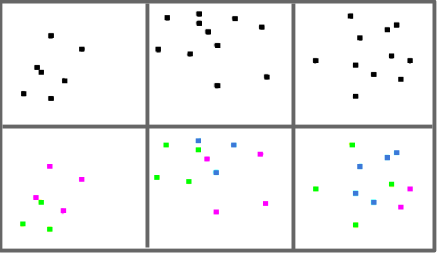
\includegraphics[width=.35\linewidth]{SCA/consinvert5}
%	\end{minipage}
%	\hfill
%	\begin{minipage}[c]{0.63\linewidth}
%		\centering
		\caption{
			Unsupervised segmentation of points belonging to up to three constellations of squares and triangles at different positions, scales and orientations. 
			The model is trained to reconstruct the points (top row) under the \gls{CCAu} mixture model. The bottom row colours the points based on the parent with the highest posterior probability in the mixture model. 
			The right-most column shows a failure case.
			Note that the model uses sets of points, not pixels, as its input; we use images  only to visualize the constellation arrangements.
		}
		\label{fig:constellations}
%	\end{minipage}
	%    \vspace*{-.75em}
\end{figure}
Empirical results show that this model is able to perform unsupervised instance-level segmentation of points belonging to different constellations, even in data which is difficult to interpret for humans. See \Cref{fig:constellations} for an example and \Cref{sec:constellation_expr} for details.
% \begin{figure}
%     \centering
%     \vspace*{.5em}
%     \begin{minipage}[b]{0.58\linewidth}
%     \centering
%     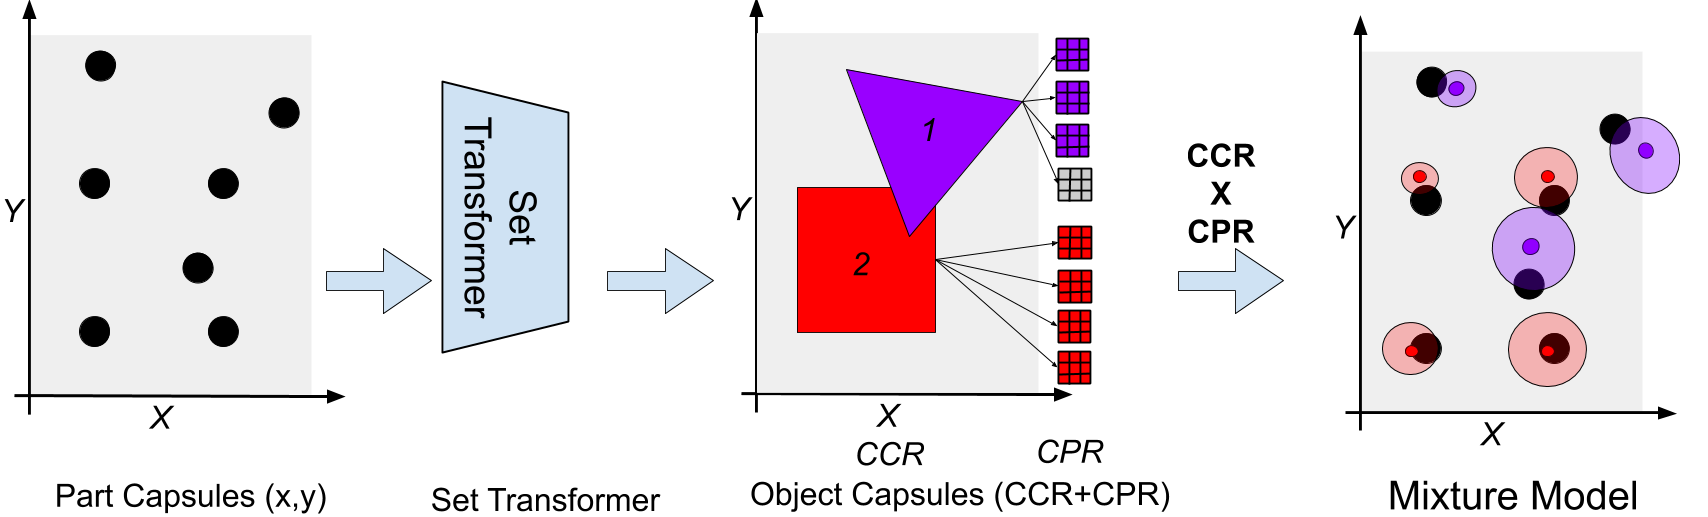
\includegraphics[width=\linewidth]{SCA/constellation_read.png}
%     \vspace*{.05em}
%     \end{minipage}
%     \hfill
%     \begin{minipage}[b]{.4\linewidth}
%     \caption{Constellation Autoencoder. 
%     The set transformer encoder $h^\mathrm{caps}$ predicts parameters of two object capsules, which predict affine transformations, precisions and presences of object and part capsules. 
%     Finally, input points are explained by a mixture of predictions, where the size of the circle corresponds to its precision.
%     }
%     \label{fig:constellation_capsule}
%     \end{minipage}
% \end{figure}

\subsection{Part Capsule Autoencoder (\textsc{pcae})}
\label{sec:img_capsule}
Explaining images as geometrical arrangements of parts requires 1) discovering what parts are there in an image and 2) inferring the relationships of the parts to the viewer (their pose).
For the \gls{CCAu} a part is just a 2D point (that is, a (x, y) coordinate), but for the \gls{PCAu} each part capsule $m$ has a six-dimensional pose $\bx_m$ (two rotations, two translations, scale and shear), a presence variable $d_m \in \interval{0, 1}$ and a unique identity.
We frame the part-discovery problem as auto-encoding: the encoder learns to infer the poses and presences of different part capsules, while the decoder learns an image template $T_m$ for each part (\cref{fig:learned_templates}) similar to \cite{Tieleman2014thesis,Eslami2016air}.
If a part exists (according to its presence variable), the corresponding template is affine-transformed with the inferred pose giving $\widehat{T}_m$.
Finally, transformed templates are arranged into the image.
% The templates corresponding to present parts are affine-transformed using their poses, and the pixels of these transformed templates are used to create a separate mixture model for each image pixel.
The \gls{PCAu} is followed by an \glsreset{OCAu}\gls{OCAu}, which closely resembles the \gls{CCAu} and is described in \Cref{sec:ocae}.

Let $\by \in \interval{0, 1}^{h \times w \times c}$ be the image.
We limit the maximum number of part capsules to $M$ and use an encoder to infer their poses $\bx_m$, presence probabilities $d_m$, and special features $\bz_m \in \RR^{c_z}$, one per part capsule.
Special features can be used to alter the templates in an input-dependent manner (we use them to predict colour, but more complicated mappings are possible). The special features also inform the \gls{OCAu} about unique aspects of the corresponding part (\!\eg occlusion or relation to other parts).
% The latter do not take part in direct image reconstruction, but inform the \gls{OCAu} about unique aspects of the corresponding part; they are trained by backpropagating derivatives from the \gls{OCAu}.
Templates $T_m \in \interval{0, 1}^{h_t \times w_t \times (c+1)}$ are smaller than the image $\by$, but have an additional alpha channel which allows occlusion by other templates. 
We use $T_m^a$ to refer to the alpha channel and $T_m^c$ to refer to its colours.

We allow each part capsule to be used only once to reconstruct an image, which means that parts of the same type are not repeated\footnote{We could repeat parts by using multiple instances of the same part capsule.}.
% At present, we do not allow multiple occurrences of the same part in an image, so the part capsules themselves are not replicated across space, though they could be.
To infer part capsule parameters we use a \gls{CNN}-based encoder followed by \textit{attention-based pooling}, which is described in more detail in the \Cref{app:attention_based_pooling} and whose effects on the model performance are analyzed in \Cref{sec:ablation}.

The image is modelled as a spatial Gaussian mixture, similarly to \cite{Greff2019multi, Burgess2019monet, Engelcke2019genesis}.
Our approach differs in that we use pixels of the transformed templates (instead of component-wise reconstructions) as the centres of isotropic Gaussian components, but we also use constant variance.
% For every pixel, we take the corresponding pixels of the transformed templates and treat them as centres of isotropic Gaussian components with constant variance.
Mixing probabilities of different components are proportional to the product of presence probabilities of part capsules and the value of the learned alpha channel for every template.
% function $f_c: \RR^c \mapsto \interval{0, 1}$ of the color value at that location\footnote{
% Templates are assumed to be sparse; if there exists a template that has a non-zero value at a given location, then these templates should be used.}
% , where $c$ is the number of image channels. 
More formally:
%\vspace*{-.3em}
% \begin{align}
%     &\bx_{1:M}, d_{1:M}, \bz_{1:M} = \operatorname{h^{\mathrm{enc}}}(\by) &\text{encode the image to part capsule parameters,}\\
%     &\bm{c}_m = \operatorname{MLP}(\bz_m) &\text{predict the color of the m$^\mathrm{th}$ template,}\\
%     &\widehat{T}_m = \operatorname{TransformImage} (T_m, \bx_m)  & \text{apply affine transforms to image templates,}\\
%     % 
%     &p^y_{m,i,j} \propto d_m \widehat{T}_{m,i,j}^a &\text{compute mixing probabilities,}\\
%     % 
%     &\p{\by} = \prod_{i,j} \sum_{m=1}^M p^y_{m,i,j}\, \gauss{y_{i,j} \mid \bm{c}_m \cdot \widehat{T}_{m,i,j}; \sigma^2_y} &\text{calculate image likelihood.} \label{eq:im_likelihood}
% \end{align}
\begin{flalign}
&\bx_{1:M}, d_{1:M}, \bz_{1:M} = \operatorname{h^{\mathrm{enc}}}(\by) &&\text{predict part capsule parameters,}\\
&\bm{c}_m = \operatorname{MLP}(\bz_m) &&\text{predict the color of the m$^\mathrm{th}$ template,}\\
&\widehat{T}_m = \operatorname{TransformImage} (T_m, \bx_m)  && \text{apply affine transforms to image templates,}\\
% 
&p^y_{m,i,j} \propto d_m \widehat{T}_{m,i,j}^a &&\text{compute mixing probabilities,}\\
% 
&\p{\by} = \prod_{i,j} \sum_{m=1}^M p^y_{m,i,j}\, \gauss{y_{i,j} \mid \bm{c}_m \cdot \widehat{T}_{m,i,j}^c; \sigma^2_y} &&\text{calculate the image likelihood.} \label{eq:im_likelihood}
\end{flalign}
% \vspace*{-.25em}
Training the \gls{PCAu} results in learning templates for object parts, which resemble strokes in the case of \textsc{mnist}, see \Cref{fig:learned_templates}.
This stage of the model is trained by maximizing the image likelihood of \Cref{eq:im_likelihood}.

\subsection{Object Capsule Autoencoder (\textsc{ocae})}
\label{sec:ocae}
% \todo{\ak{explain why constellation and object aes are differnet}}

\begin{figure}
	\centering
%	\begin{minipage}[c]{.7\linewidth}
		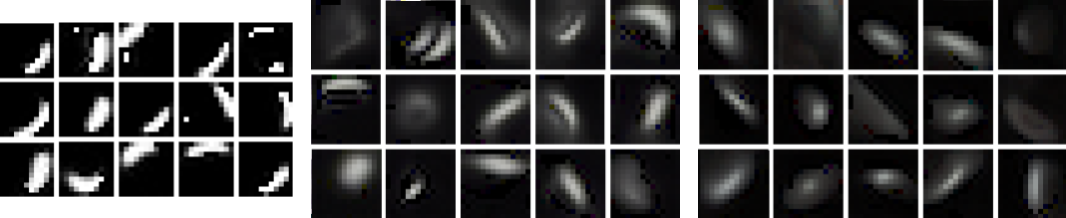
\includegraphics[width=.7\linewidth]{SCA/templates}
		%    \vspace*{.25em}
%	\end{minipage}
%	\hfill
%	\begin{minipage}[c]{.29\linewidth}
		\caption{Stroke-like templates learned on \textsc{mnist} (left) as well as sobel-filtered \textsc{svhn} (middle) and \textsc{cifar10} (right).
			For \textsc{svhn} they often take the form of double strokes due to sobel filtering.
			% , which effectively extracts edges.
		}
		\label{fig:learned_templates}
%	\end{minipage}
\end{figure}
\begin{figure}
	\centering
	\begin{subfigure}[c]{.06\linewidth}
		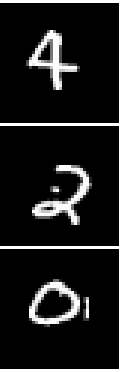
\includegraphics[width=\linewidth]{SCA/mnist/inputs}
		\caption{}
	\end{subfigure}
	% \hfill
	\begin{subfigure}[c]{.06\linewidth}
		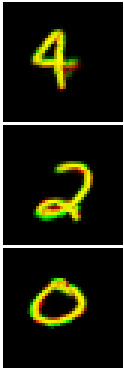
\includegraphics[width=\linewidth]{SCA/mnist/recs}
		\caption{}
	\end{subfigure}
	% \hfill
	\begin{subfigure}[c]{.03967\linewidth}
		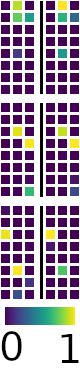
\includegraphics[width=\linewidth]{SCA/mnist/acts}
		\caption{}
	\end{subfigure}
	% \hfill
	\begin{subfigure}[c]{.12\linewidth}
		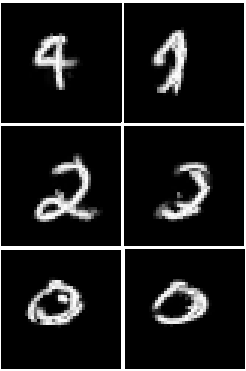
\includegraphics[width=\linewidth]{SCA/mnist/caps_recs}
		\caption{}
	\end{subfigure}
	% \hfill
	\begin{subfigure}[c]{.30\linewidth}
		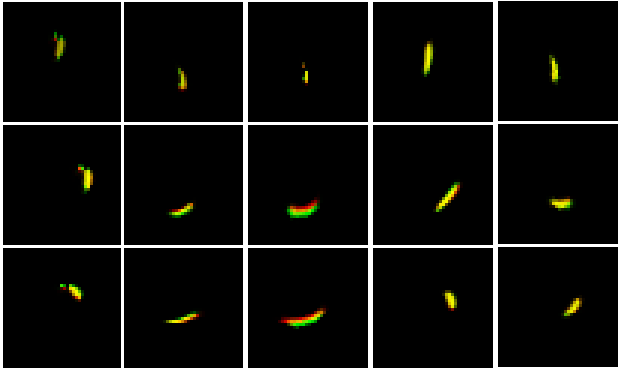
\includegraphics[width=\linewidth]{SCA/mnist/transformed_templates}
		\caption{}
	\end{subfigure}
%	\begin{minipage}[c]{.35\linewidth}
		\caption{
			% $40\times40$ 
			\textsc{Mnist} (a) images, (b) reconstructions from part capsules in red and object capsules in green, with overlapping regions in yellow.
			Only a few object capsules are activated for every input (c) a priori (left) and even fewer are needed to reconstruct it (right).
			The most active capsules (d) capture object identity and its appearance;
			(e) shows a few o  f the affine-transformed templates used for reconstruction.
		}
		\label{fig:mnist_rec}
%	\end{minipage}
\end{figure}

Having identified parts and their parameters, we would like to discover objects that could be composed of them\footnote{
	Discovered objects are {\it not} used top-down to refine the presences or poses of the parts during inference. However, the derivatives backpropagated via \gls{OCAu} refine the lower-level encoder network that infers the parts.
}.
To do so, we use concatenated poses $\bx_m$, special features $\bz_m$ and flattened templates $T_m$ (which convey the identity of the part capsule)
as an input to the \gls{OCAu}, which differs from the \gls{CCAu} in the following ways.
Firstly, we feed part capsule presence probabilities $d_m$ into the \gls{OCAu}'s encoder---these are used to bias the Set Transformer's attention mechanism not to take absent points into account.
% ; see \Cref{app:set_transformer} for details.
Secondly, $d_m$s are also used to weigh the part-capsules' log-likelihood, so that we do not take log-likelihood of absent points into account. 
This is implemented by raising the likelihood of the m$^\mathrm{th}$ part capsule to the power of $d_m$, \textit{cf}. \Cref{eq:constellation_likelihood}.
Additionally, we stop the gradient on all of \gls{OCAu}'s inputs except the special features to improve training stability and avoid the problem of collapsing latent variables; see\eg \cite{Rasmus2015ladder}.
Finally, parts discovered by the \gls{PCAu} have independent identities (templates and special features rather than 2D points).
Therefore, every part-pose is explained as an independent mixture of predictions from object-capsules---where every object capsule makes exactly $M$ candidate predictions $\mu_{k,1:M}$, or exactly {\bf one} candidate prediction per part.
Consequently, the part-capsule likelihood is given by,
%\vspace*{-.5em}
% \begin{equation}
%     \p{\bx_{1:M}} = \prod_{m=1}^M \sum_{k=1}^K  
%     \frac{a_k a_{k,m}}{\sum_i a_i \sum_j a_{i,j}}
%     \,\p{\bx_m}{k,m}\,. \label{eq:mod_constellation_likelihood}
% \end{equation}
\begin{equation}
\p{\bx_{1:M}, d_{1:M}} = \prod_{m=1}^M \left[\, \sum_{k=1}^K  
\frac{a_k a_{k,m}}{\sum_i a_i \sum_j a_{i,j}}
\,\p{\bx_m}{k,m}\right]^{d_m}\,. \label{eq:mod_constellation_likelihood}
\end{equation}
The \gls{OCAu} is trained by maximising the part pose likelihood of \Cref{eq:mod_constellation_likelihood}, and it learns to discover further structure in previously identified parts, leading to learning sparsely-activated object capsules, see \Cref{fig:mnist_rec}.
Achieving this sparsity requires further regularization, however.

\subsection{Achieving Sparse and Diverse Capsule Presences}
\label{sec:losses}
Stacked Capsule Autoencoders are trained to maximise pixel and part log-likelihoods ($\loss[\mathrm{ll}]{} = \log\p{\by} + \log\p{\bx_{1:M}}$).
If not constrained, however, they tend to either use all of the part and object capsules to explain every data example or collapse onto always using the same subset of capsules, regardless of the input.
We want the model to use different sets of part-capsules for different input examples and to specialize object-capsules to particular arrangements of parts. 
To encourage this, we impose sparsity and entropy constraints.  We evaluate their importance in \Cref{sec:ablation}.

We first define prior and posterior object-capsule presence as follows.
For a minibatch of size {\small$B$} with {\small$K$} object capsules and $M$ part capsules we define a minibatch of prior capsule presence $a^\mathrm{prior}_{1:K}$ with dimension {\small$[B, K]$} and posterior capsule presence $a^\mathrm{posterior}_{1:K,1:M}$ with dimension {\small$[B, K, M]$} as,
%\vspace*{-.2em}
\begin{equation}
a^\mathrm{prior}_k = a_k \max_m a_{m,k}\,,
\qquad
a^\mathrm{posterior}_{k,m} = a_k a_{k,m}\;\gauss{\bx_m \mid m,k}\,,
\end{equation}
respectively; the former is the maximum presence probability among predictions from object capsule $k$ while the latter is the unnormalized mixing proportion used to explain part capsule~$m$.
%\vspace*{-.5em}
\begin{description}[leftmargin=\parindent]
	\item[Prior sparsity]
	Let $\overline{u}_k = \sum_{b=1}^B a^\mathrm{prior}_{b,k}$ the sum of presence probabilities of the object capsule $k$ among different training examples, and $\widehat{u}_b = \sum_{k=1}^K a^\mathrm{prior}_{b,k}$ the sum of object capsule presence probabilities for a given example.
	If we assume that training examples contain objects from different classes uniformly at random and we would like to assign the same number of object capsules to every class, then each class would obtain $\nicefrac{K}{C}$ capsules.
	Moreover, if we assume that only one object is present in every image, then $\nicefrac{K}{C}$ object capsules should be present for every input example, which results in the sum of presence probabilities of $\nicefrac{B}{C}$ for every object capsule.
	To this end, we minimize, 
	% \todo{\ak{which means that each obj capsule should be activated with $\nicefrac{1}{C}$ probability, and the $B$ in the numerator is a bug}}
	%    \vspace*{-.75em}
	\begin{equation}
	\loss[\mathrm{prior}]{} = 
	\frac{1}{B} \sum_{b=1}^B \left(\widehat{u}_b  - \nicefrac{K}{C} 
	\right)^2
	+
	\frac{1}{K} \sum_{k=1}^K \left(\overline{u}_k  - \nicefrac{B}{C} \right)^2\,. \label{eq:prior_sparsity}
	\end{equation}
	% 
	\item[Posterior Sparsity]
	Similarly, we experimented with minimizing the within-example entropy of capsule posterior presence $\mathcal{H}(\overline{v}_k)$ and maximizing its between-example entropy $\mathcal{H}(\widehat{v}_b)$, where $\mathcal{H}$ is the entropy, and where $\overline{v}_k$ and $\widehat{v}_b$ are the the normalized versions of  $\sum_{k,m} a^\mathrm{posterior}_{b,k,m}$
	and $\sum_{b,m} a^\mathrm{posterior}_{b,k,m}$, respectively.
	The final loss reads as
	\begin{equation}
	\loss[\mathrm{posterior}]{} = \frac{1}{K} \sum_{k=1}^K \mathcal{H}(\overline{v}_k) - \frac{1}{B} \sum_{b=1}^B \mathcal{H}(\widehat{v}_b)\,. \label{eq:posterior_sparsity}
	\end{equation}
	Our ablation study has shown, however, that the model can perform equally well without these posterior sparsity constraints, cf. \Cref{sec:ablation}.
	%    
	%    Similarity, let $\overline{v}_k$ and $\widehat{v}_b$ be the the normalized versions of  $\sum_{k,m} a^\mathrm{posterior}_{b,k,m}$
	%    and $\sum_{b,m} a^\mathrm{posterior}_{b,k,m}$, respectively.
	%    We find it beneficial to minimize the within-example entropy of capsule posterior presence $\mathcal{H}(\overline{v}_k)$ and maximize its between-example entropy $\mathcal{H}(\widehat{v}_b)$, where $\mathcal{H}$ is the entropy \todo{\ak{say why it is beneficial}}. The final loss reads as,
	%%    \vspace*{-1.25em}
	%    \begin{equation}
	%        \loss[\mathrm{posterior}]{} = \frac{1}{K} \sum_{k=1}^K \mathcal{H}(\overline{v}_k) - \frac{1}{B} \sum_{b=1}^B \mathcal{H}(\widehat{v}_b)\,. \label{eq:posterior_sparsity}
	%    \end{equation}
	%
\end{description}
\begin{figure}
	\centering
	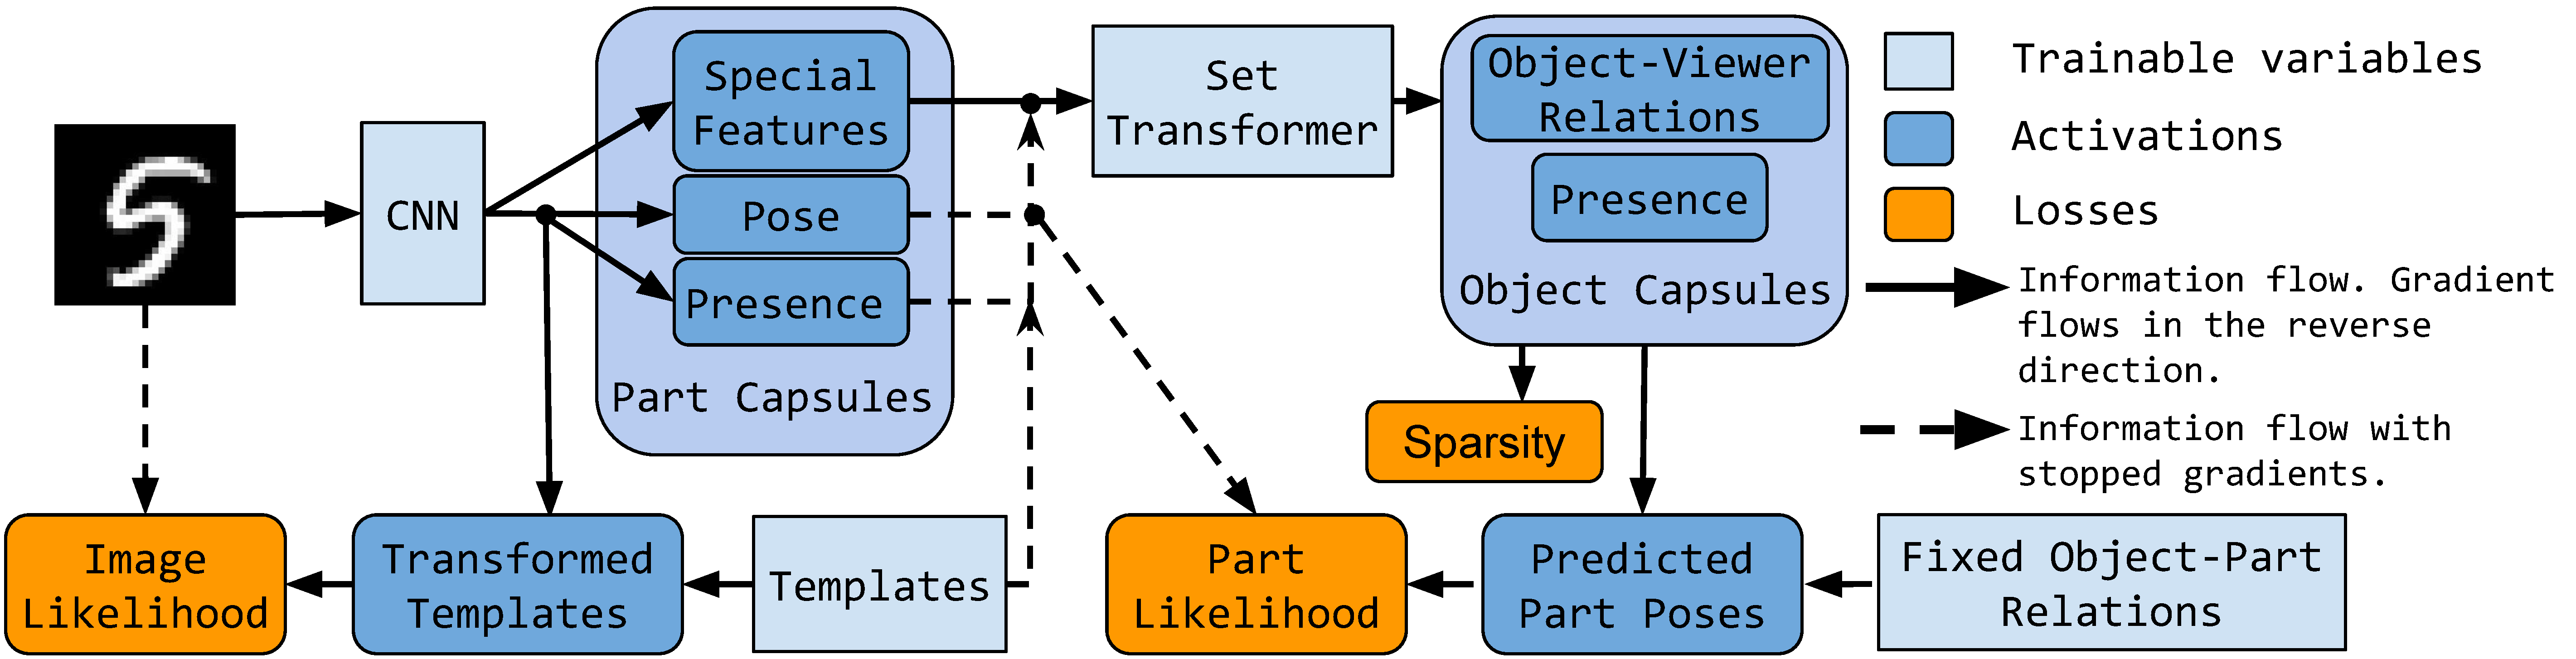
\includegraphics[width=\linewidth]{SCA/sca_architecture_v3}
	\caption{\gls{SCAu} architecture.}
	\label{fig:sca_arch}
\end{figure}
\cref{fig:sca_arch} shows the schematic architecture of \gls{SCAu}. We optimize a weighted sum of image and part likelihoods and the auxiliary losses. 
Loss weight selection process, as well as the values used for experiments, are detailed in \Cref{app:models}.

In order to make the values of presence probabilities ($a_k, a_{k,m}$ and $d_m$) closer to binary we inject uniform noise $\in \interval{-2, 2}$ into logits, similar to \cite{Tieleman2014thesis}.
This forces the model to predict logits that are far from zero to avoid stochasticity and makes the predicted presence probabilities close to binary.
Interestingly, it tends to work better in our case than using the Concrete distribution \citep{Maddison2017concrete}.